\section{System Architecture}

This system mainly focus in the interconnection and interoperability of different elements. 
To achieve this, an architecture was designed in response to the requirements.

A general overview of the proposed architecture can be seen in \autoref{fig:architecture}.

\begin{figure}[H]
    \centering
    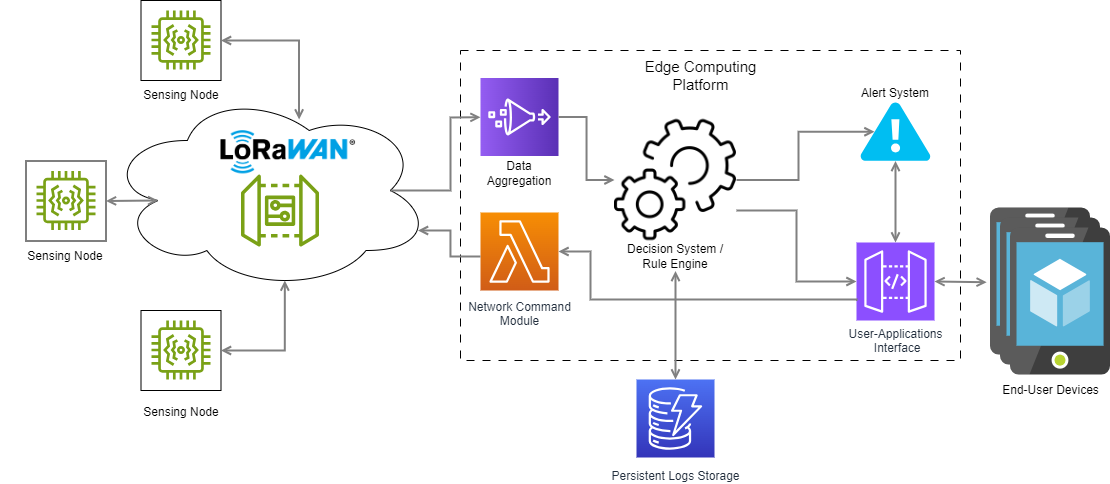
\includegraphics[width=1\textwidth]{./images/7/generalArchitecture.png}
    \caption{General architecture design for the proposed system.}
    \label{fig:architecture}
\end{figure}

Thanks to the research done, the selection for the intercommunication of the nodes with the edge platform 
will be done using \acrshort{lorawan}. This protocol ensures good coverage in rural areas, moreover, it ensures 
scalability in the system designed. The connection is done with lora from the nodes to the gateway. 
This gateway connects to the edge computing platform with IP technologies to send all the data from the nodes. 
Finally, this data will be collected in the data aggregation module, which will allow information coming from other 
wireless technologies or other \acrfullr{lln}.

When all the data is aggregated, it will pass through the rule engine module. This step analyzes the data in search 
for patterns that indicate the existence of a fire or will animal near the system. All these processing is logged into a 
persistent data storage that can serve as a knowledge base for future projects. 

If a fire or wild animal is detected, a set of actions are done, this is done through the alarm system of the edge platform and 
the User-Application interface. These modules allows for interaction with the users, allowing different functionalities like:
\begin{itemize}
    \item Access from mobile applications to the processed data.
    \item Real-Time alarm and registration of events.
    \item Allowing users to react, sending commands to the network to solve problems.
\end{itemize}

